% Chapter Template

\chapter{Learning} % Main chapter title

\label{Chapter 4} % Change X to a consecutive number; for referencing this chapter elsewhere, use \ref{ChapterX}

\lhead{Chapter 4. \emph{Learning}} % Change X to a consecutive number; this is for the header on each page - perhaps a shortened title

It is then possible to learn the parameters of the CPG to optimize the movement of the structure. Instead of having to find the value of the angles, the CPGs act as basis function for the angles, and thatway we reduce the space of research to a space with finite dimensions. All the parameters (frequency, offset and amplitude of each node) are scaled to fit between $0$ and $1$. A simple fitness function can be extracted from the simulation, for example the distance traveled by the head of the structure. 

It is not possible to get a gradient or Hessian matrix for this problem, as the function comes from the simulation. Moreover, the fitness function is not likely to be convex, as taking the mean of two good solutions for the movement of a structure does not necessary provide a good solution. The fitness function can also present some discontinuities or high variations because of collisions. Collisions are not continuous phenomena and even if the physics engine use smoothing techniques to simplify interractions, there is a very small difference between a biped structure walking and a biped structure almost walking but with one leg that does not touch the ground, but the fitness function will give completely different results as one structure is moving and the other is not. Finally there is also the problem of consistency of a result, because two structures can behave differently for the same parameters, as the simulation can show chaotic behavior as small variations can have a big impact on the movement. For all these reasons, it is difficult to use classical optimisation for the creatures to learn how to move in the simulated environment. 

\begin{figure}[htbp]
    \centering
    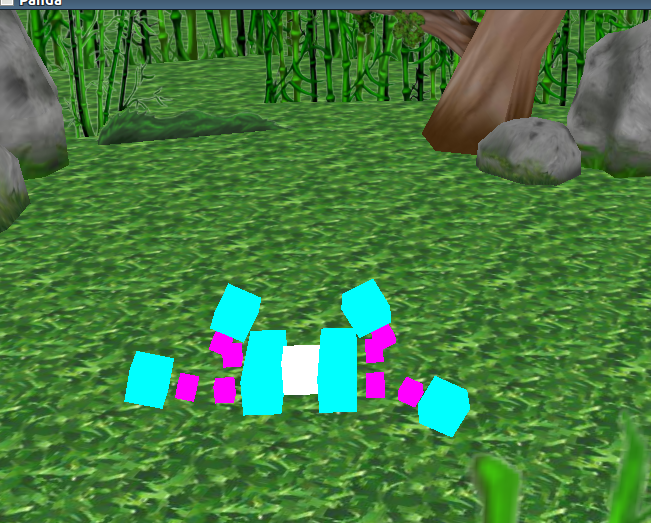
\includegraphics[scale=0.5]{Figures/four_legged.png}
    \rule{35em}{0.5pt}
    \caption[A structure with four legs learning]{A structure with four legs learning}
    \label{fig:four_legged}
\end{figure}

\section{Random Search}

A first very simple way of finding good solution is random search. We test a random set of parameters and keep the vector of parameters showing the best results. This has the benefit of being very simple to implement and provides a good testbench for fixing issues with the simulation. A first problem observed was the consistency of the solution, testing the same parameters can lead to very different results. A first way to correct this was to take longer sample (about 20 sec of simulation). Even with this correction, online learning brought some issues, as it is possible that a good results is only good because of the initial configuration given by testing previous movement. A way to correct this is to set all angles to a default value and wait for the structure to be have a null velocity. This also led to some issues and showed solution using the first movement to jump as far as poissible. 

\section{Nelder-Mead method}

The Nelder Mead method (or downhill simplex method) is a way of finding a local optimum, without knowing the gradient of the function in a given multidimensional space. We initialize a non-degenerated simplex in this space, then we follow this procedure (source: wikipedia):
\begin{itemize}
    \item Ordering: we order the points of the simplex such that $f(x_0) >= f(x_1) >= f(x_2) \dot >= f(x_n)$, where f is the fitness function that we want to maximize ( traveled distance...)
    \item We compute the center of gravity of all the points $x_g$

    \item We compute the reflection of $x_n$ in respect to $x_g$ ($x_r = x_g + (x_g - x_n )$)

    \item If $f(x_r) > f(x_{n - 1})$ then we compute the expansion point : $x_e = x_g + 2 * (x_g - x_n )$ if $f(x_e) > f(x_r)$ we replace $x_n$ with $x_e$ else $x_r$ and we go back to the first step.

    \item If $f(x_r) > f(x_{n - 1})$ then we compute the contraction point : $x_c = x_g + 0.5 * (x_g - x_n )$ if $f(x_c) > f(x_n)$ we replace $x_n$ with $x_c$ and go back to the first step, else we do the next step

    \item a contraction homotethia of center $x_0$ : we replace $x_i$ with : $x_i = x_0 + 0.5 * (x_i - x_0 )$ for $i > 0$ and go back to the first step.
\end{itemize}
 
\begin{figure}[htbp]
    \centering
    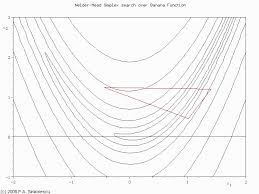
\includegraphics[scale=0.7]{Figures/nelder_mead.jpg}
    \rule{35em}{0.5pt}
    \caption[A simplex following the Nelder-Mead method]{A simplex following the Nelder-Mead method}
    \label{fig:nelder_mead}
\end{figure}


This method gave some good results for simple creature, (without to many degrees of freedom). I modified it to evaluate the function again, each time we sort the points of the simplex. Though it is less efficient, thatway, it is possible to prevent from having a lucky trial. For instance, as the test depends of initial condition, sometimes a result can be really good, but cannot be repeated, for instance a four legged structure can get a good score but end up on the back after one trial and will not be efficient on the next ones.

